\documentclass{beamer}

\usepackage{listings}
\usepackage{color}
\definecolor{atomPurple}{RGB}{198,120,221}
\definecolor{atomRed}{RGB}{224,108,117}
\definecolor{atomGreen}{RGB}{152,195,121}
\definecolor{atomGreyLight}{RGB}{171,178,191}
\definecolor{atomGreyDark}{RGB}{92,99,112}
\definecolor{atomBlack}{RGB}{56,58,66}

\lstset{
language=C,
numbers=left,
showstringspaces=false,
tabsize=4,
keywordstyle=\color{atomPurple},
stringstyle=\color{atomGreen},
commentstyle=\color{atomGreyDark}
}

\title{Better Software Development Through Automated Tooling}
\author{Vaughan Kitchen}
\date{April 28, 2017}

\begin{document}

\begin{frame}
\titlepage
\end{frame}

\begin{frame}{Structure}
\begin{itemize}
	\item Background
	\item Survey of Tools
	\item Live Demonstration
	\item Project Examples
	\item Related Topics
\end{itemize}
\end{frame}

\begin{frame}{Background}
	\begin{block}{What}
		Plug as many automatic tools as possible into the development of JASSv2
		(A search enging being developed by Andrew Trotman)
	\end{block}
	\begin{block}{When}
		A summer studentship at the start of 2017
	\end{block}
	\begin{block}{How}
		The approach was to first figure out what tools we might want. Then what
		tools were available to us. Which of the available ones were worth
		integrating. And then get them integrated
	\end{block}
\end{frame}

\begin{frame}{An Overview of Tools}
	\begin{itemize}
		\item Unit Tests
		\item Integration Tests
		\item System Tests
		\item Regression Tests
		\item Code Coverage
		\item Static Analysis
		\item Memory \& Leak Checks
		\item Performance Profiling
		\item Code Hygiene
		\item Code Documentation
	\end{itemize}
\end{frame}

\begin{frame}{Continuous Integration pt.1}
	Travis CI
	\begin{itemize}
		\item Automates Build
		\item Integrates with Github (or BitBucket for some CI systems)
		\item Runs on every push
		\item An hour of compute time per VM instance
		\item What else can it do besides build?
	\end{itemize}
\end{frame}

\begin{frame}{Unit Testing 1}
	
\includegraphics[width=\linewidth]{unit-test.jpeg}
\end{frame}

\defverbatim[colored]\lstI{\begin{lstlisting}
#include "unity.h"
#include "string2.h"

void test_string_append(void)
	{
	/* test the normal use case */
	struct string *s = string_new_c("cat");
	string_append_c(s, "dog");
	TEST_ASSERT_EQUAL_STRING(s->str, "catdog");
	TEST_ASSERT_EQUAL_UINT(s->bytes, 6);

	string_free(s);
	}
\end{lstlisting}
}

\begin{frame}{Unit Testing 2}
	\lstI
\end{frame}

\begin{frame}{Unit Testing 3}
	\begin{tabular}{cl}
		\begin{tabular}{c}
			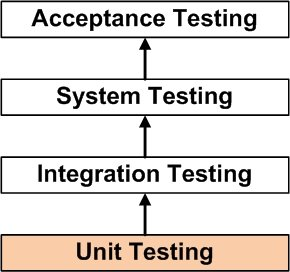
\includegraphics[width=100px]{unittesting.jpg}
		\end{tabular}
	&
		\begin{tabular}{l}
			\parbox{0.5\linewidth}{
				\begin{itemize}
					\item If it isn't tested, it doesn't work
					\item Part of your test suite
					\item Runs from your Continuous Integration system
					\item Assures the quality of individual units
					\item Smallest testable unit (Function, or Class)
					\item Simplifies integration
					\item Confidence in refactoring
					\item Provides documentation
					\item JUnit, CUnit, Unity, tinytest, Jasmine...
				\end{itemize}
			}
		\end{tabular}
	\end{tabular}
\end{frame}

\begin{frame}{Test Driven Development}
	\begin{itemize}
		\item How do you know when you're finished?
		\item Do you know what you're building?
		\item How far through building it are you?
		\item Refactor mercilessly
		\item Type systems can't always save you
	\end{itemize}
\end{frame}

\begin{frame}{Integration Testing}
	\begin{tabular}{cl}
		\begin{tabular}{c}
			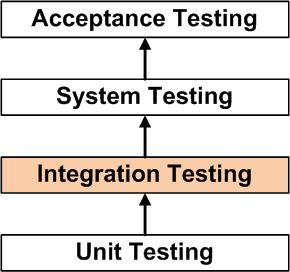
\includegraphics[width=100px]{integrationtesting.jpg}
		\end{tabular}
	&
		\begin{tabular}{l}
			\parbox{0.5\linewidth}{
				\begin{itemize}
					\item Part of your test suite
					\item Runs from your Continous Integration system
					\item Next step up from unit tests
					\item Tests whether groups of modules work together correctly
					\item Doesn't test the correctness of the system as a whole
				\end{itemize}
			}
		\end{tabular}
	\end{tabular}
\end{frame}

\begin{frame}{System Testing}
	\begin{tabular}{cl}
		\begin{tabular}{c}
			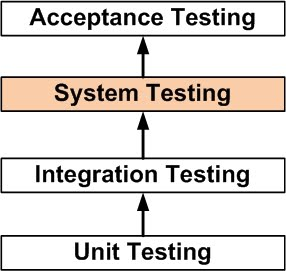
\includegraphics[width=100px]{system_testing.jpg}
		\end{tabular}
	&
		\begin{tabular}{l}
			\parbox{0.5\linewidth}{
			\begin{itemize}
				\item Does the application do what it should?
				\item Hard to automate entirely
				\item Can automate some code paths (CI has full power of Linux)
				\item bats (Bash Automated Testing System)
			\end{itemize}
			}
		\end{tabular}
	\end{tabular}
\end{frame}

\begin{frame}{Regression Testing}
	\begin{itemize}
		\item Does the previously functional software still function correctly?
		\item Computing power is now cheap
		\item Run the entire test suite for each push
		\item Continuous Integration system will notify on breakage
		\item Regression tests are now free
	\end{itemize}
\end{frame}

\begin{frame}{Code Coverage}
	
\includegraphics[width=100px]{codecov.png}
	\begin{itemize}
		\item How much of the source code does the test suite execute?
		\item Do tests cover succeeding and failing paths?
		\item Function coverage
		\item Statement coverage
		\item Branch coverage
		\item Condition coverage
		\item Codecov, Coveralls
	\end{itemize}
\end{frame}

\begin{frame}{Static Analysis}
	
\includegraphics[width=100px]{coverity.png}
	\begin{itemize}
		\item Verify behaviour
		\item Lint for best practices
		\item Prove correctness
		\item Sometimes freely available to Open Source projects
		\item Can be integrated into CI
	\end{itemize}
\end{frame}

\begin{frame}{memcheck}
	\begin{itemize}
		\item Dynamic analysis
		\item Memory leaks
		\item Corrupted memory
		\item Valgrind
	\end{itemize}
\end{frame}

\begin{frame}{Performance Profiling}
	\begin{itemize}
		\item Algorithmic performance
		\item Web performance
		\item Responsive vs Throughput
		\item Part of regression testing
		\item Instrumentation, Sampling
		\item Gprof, Callgrind
	\end{itemize}
\end{frame}

\begin{frame}{Code Hygiene}
	\begin{itemize}
		\item Code smell
		\item Linting
		\item Best Practices
		\item Anti-patterns
		\item CodeClimate, CodeLingo
	\end{itemize}
\end{frame}

\begin{frame}{Code Documentation}
	\begin{itemize}
		\item Doxygen, Javadoc
		\item CodeDocs.xyz
		\item GitHub Pages
	\end{itemize}
\end{frame}

\begin{frame}{Continuous Integration pt.2}
	\begin{itemize}
		\item Merge all working copies to mainline several times a day
		\item Prevents "integration hell"
		\item Feature toggles for partially complete code
		\item Continuous Delivery (mainline is always in a deployable state)
		\item Continuous Deployment (automatic deployment to production)
		\item Notify the developer that broke the code (default) or specified manager/team
	\end{itemize}
\end{frame}

\begin{frame}{YAML 1}
	\begin{itemize}
		\item Superset of JSON
		\item Supports comments
		\item Often used as a configuration format
	\end{itemize}
\end{frame}

\defverbatim[colored]\lstII{\begin{lstlisting}
"object": {
	"key": "value",
	"array": [
		{
			"null_value": null
		},
		{
			"boolean": true
		},
		{
			"integer": 1
		},
		{
			"string": "rope"
		}
	]
}
\end{lstlisting}
}

\begin{frame}{YAML 2}
	\lstII
\end{frame}

\defverbatim[colored]\lstIII{\begin{lstlisting}
object:
	key: value
  array:
    - null_value:
    - boolean: true
    - integer: 1
		- string: rope
\end{lstlisting}
}

\begin{frame}{YAML 3}
	\lstIII
\end{frame}

\begin{frame}{Our Set Up}
	\begin{itemize}
		\item Travis CI (OSX, and Linux)
		\item AppVeyor (Windows)
		\item Unit Testing in a custom framework
		\item Coverity (coverity\_scan branch)
		\item Valgrind
		\item CodeCov (Gcov)
		\item CodeDocs.xyz (integrates directly with GitHub)
	\end{itemize}
\end{frame}

\begin{frame}{Live Demonstration}
\end{frame}

\begin{frame}{Other Set Ups}
	\begin{itemize}
		\item https://github.com/DandyHQ/mace-prototype
		\item https://github.com/rubinius/rubinius
		\item https://github.com/IronLanguages/main
	\end{itemize}
\end{frame}

\begin{frame}{Continuous Deployment}
	\begin{itemize}
		\item Next step from Continuous Delivery
		\item Code automatically deployed to production
		\item Seen in SAAS or Web Applications
		\item Application monitoring and Dashboards
		\item Feature Toggles
		\item Graphs and anomoly detection
	\end{itemize}
\end{frame}

\begin{frame}{Property Based Testing}
	Fuzzing
	\begin{itemize}
		\item Runs the program against random input
		\item Used to check for security vulnerabilities
		\item American Fuzzy Lop (AFL) uses genetic algorithms and instrumentation to try and reach all code paths
	\end{itemize}
	Property Based Testing
	\begin{itemize}
		\item Unit Testing on roids
		\item Do properties of the output still hold when the program is run with random input
		\item Forces the consideration of edge cases
		\item Reduces failures to minimal counter examples
		\item QuickCheck, ScalaCheck, ClojureCheck, JavaQuickCheck, RapidCheck (C++)
	\end{itemize}
\end{frame}

\begin{frame}{Roll Your Own}
	Webhooks
	\begin{itemize}
		\item Webhooks form the foundation of integrations
		\item Subscribe to specific events
		\item push, fork, issues, release, watch...
		\item HTTP POST payload to specified URL
		\item Secure your webhook with a secret token, payloads will be signed
	\end{itemize}
	Other APIs
	\begin{itemize}
		\item There is also an integration API to give applications access to private repositories etc.
		\item OAuth application is authenticated as if it's the user
	\end{itemize}
\end{frame}

\begin{frame}{Attributions}
	\begin{itemize}
		\item http://softwaretestingfundamentals.com Testing images, used under CC Attribution-ShareAlike
	\end{itemize}
\end{frame}

\end{document}
